\documentclass{beamer}
\usepackage{beamerthemesplit}
\usepackage{graphics}
\logo{
\includegraphics[height=1cm]{psi_logo_white.png}}
\usetheme{Pittsburgh}
\usecolortheme{dove}
\beamertemplatenavigationsymbolsempty
\setbeamertemplate{footline}[frame number]
\definecolor{myback}{RGB}{175,238,238}
\setbeamercolor{structure}{bg=myback}
\usepackage[T1]{fontenc}
\newcommand{\changefont}[3] {
 \fontfamily{#1} \fontseries{#2} \fontshape{#3} \selectfont}

\title{NeXus Recapitulation and Developments}
\author{Mark K\"onnecke }
\institute{NeXus International Advisory Committee}
\date{\today} 

\begin{document}

\begin{frame}
\titlepage
\end{frame}

\begin{frame}
\frametitle{The Predicament of the Traveling Scientist}
\begin{itemize}
\item<1->A different data format wherever she goes
\item<2->Spends lots of time converting formats or writing readers
\item<3->Waits even longer to load data from inefficient data formats
\item<4->DA requires N files in different  formats, notes, local knowledge 
\item<5->Cannot read her collaborators data
\item<6->Has to keep extra information in yet another form
\end{itemize}
\end{frame}

\begin{frame} \frametitle{NeXus Mission}
\begin{itemize}
\item Definition of a standard data format
\begin{itemize}
\item Rules
\item Validation tools
\end{itemize}
\item Promotion of NeXus
\begin{itemize}
\item Documentation
\item NeXus API
\item Outreach to the scientific community
\end{itemize}
\end{itemize}
\end{frame}

\begin{frame} \frametitle{NeXus Design}
\begin{itemize}
\item Complete data for typical use
\item Extendable, add additional data as you please
\item Self describing
\item Easy automatic plotting
\item Platform independent, public domain, efficient
\item Suitable for a wild variety of applications
\end{itemize}
\end{frame}

\begin{frame}
 \frametitle{NeXus Levels }
\begin{enumerate}
\item Physical file format and API for accessing files
\item Rules for storing data in files
\item Component and application definitions
\item NeXus Utilities
\end{enumerate}
\end{frame}

\begin{frame} \frametitle{Physical File Format }
\begin{itemize}
\item Portable, self describing, extendable, public domain
\item Hierarchical data format, NCSA, HDF-4, later HDF-5
\item HDF-5:
\begin{itemize}
\item grouping support
\item on the fly compression
\item reading/writing subsets
\item first dimension appendable
\item Public domain C, F77 access library
\item Used by: NASA, Boing, the weathermen, .... 
\end{itemize}
\item XML for those who wish to edit their data
\end{itemize}
\end{frame}


\begin{frame} \frametitle{NeXus API }
\begin{itemize}
\item NeXus-API hides complex HDF API
\item Transparent access to all three supported physical file formats
\item ANSI-C implementation
\item Bindings: F77, Java, SWIG
\item January, 4, 2010: 1311217 files processed at PSI alone
\item {\color{red}NEW}: first class bindings to C++, python, IDL
\end{itemize}
\end{frame}


\begin{frame} \frametitle{NeXus Objects}
\begin{itemize}
\item Files
\item Groups identified by name and a classname beginning with NX
\item Scientific data sets
\item Attributes
\item Links
\end{itemize}
\end{frame}


\begin{frame} \frametitle{NeXus Raw Data File Structure}
\begin{tabbing}
\hspace*{1cm} \= \hspace*{1cm} \= \hspace*{1cm} \= \hspace*{1cm} \= \hspace*{1cm} \= \hspace*{1cm}\= \kill
entry:NXentry \\
 \>sample:NXsample \\
\\
 \>instrument:NXinstrument\\
 \> \> source:NXsource\\
 \> \> velocity\_selector:NXvelocity\_selector\\
 \> \> detector:NXdetector \\
 \> \> \>data[xsize,ysize], signal=1 (1)\\
 \>control:NXmonitor\\
 \> \>data\\
 \>data:NXdata\\
 \> \> link to (1)\\
\end{tabbing}
\end{frame}

\begin{frame} \frametitle{NeXus Processed Data File Structure}
\begin{tabbing}
\hspace*{1cm} \= \hspace*{1cm} \= \hspace*{1cm} \= \hspace*{1cm} \= \hspace*{1cm} \= \hspace*{1cm}\= \kill
entry:NXentry \\
 \>sample:NXsample \\
 \>processing\_name:NXprocess\\
 \> \>program \\
 \> \>version \\
 \> \>parameters:NXparameter \\
 \> \> \>raw\_file \\
 \>data:NXdata\\
 \> \> data[nx,ny,nz], signal=1\\
\end{tabbing}
\end{frame}

\begin{frame} \frametitle{Why the Hierarchy??}
\begin{itemize}
\item<1->Supports self description and allows short names in components
\item<2->Name, classname pair allows for multiple components of the same type
\item<3->NXentry allows for multiple datasets in the same file
\item<4->NXdata supports automatic plotting
\item<5->Take care once when writing, use n times
\end{itemize}
\end{frame}

\begin{frame}
\frametitle{Scans}
\begin{itemize}
\item Come in all shapes and sizes
\item Captured by rules:
\begin{itemize}
\item Store all varied parameters as arrays of length NP at the appropriate place in the NeXus 
 hierarchy
\item For multi detectors, NP, number of scan points is always the first dimension
\item In NXdata: create links to counts and varied variables
\end{itemize}
\end{itemize}
\end{frame}


\begin{frame}
\frametitle{Scan Example 1: rotating sample}

\begin{tabbing}
\hspace*{1cm} \= \hspace*{1cm} \= \hspace*{1cm} \= \hspace*{1cm} \= \hspace*{1cm} \= \hspace*{1cm}\= \kill
entry:NXentry \\
 \>sample:NXsample\\
 \> \> rotation\_angle[NP], axis=1 (1) \\
 \> instrument:NXinstrument\\
 \>  \>detector:NXdetector\\
 \>  \> \>data[NP],signal=1 (2)\\
 \>control:NXmonitor\\  
 \> \>data[NP]\\  
 \>data:NXdata\\
 \> \> link to (1)\\
 \> \> link to (2) \\
\end{tabbing}
\end{frame}

\begin{frame}
\frametitle{Scan Example 2: complex scan in Q}

\begin{tabbing}
\hspace*{1cm} \= \hspace*{1cm} \= \hspace*{1cm} \= \hspace*{1cm} \= \hspace*{1cm} \= \hspace*{1cm}\= \kill
entry:NXentry \\
 \>sample:NXsample\\
 \> \> rotation\_angle[NP], axis=1 (1) \\
 \> \> phi[NP], axis=1 (2) \\
 \> \> chi[NP], axis=1 (3) \\
 \> \> h[NP], axis=1 (4), primary=1 \\
 \> \> k[NP], axis=1 (5) \\
 \> \> l[NP], axis=1 (6) \\
 \> instrument:NXinstrument\\
 \>  \>detector:NXdetector\\
 \>  \> \>data[NP],signal=1 (7)\\
 \>  \> \>polar\_angle[NP],signal=1 (8)\\
 \>data:NXdata\\
 \> \> link to (1)\\
 \> \> link to (2) \\
 \> \> link to (...) \\
 \> \> link to (8) \\
\end{tabbing}
\end{frame}


\begin{frame}
\frametitle{Scan Example 3: sample rotation, area detector}
\begin{tabbing}
\hspace*{1cm} \= \hspace*{1cm} \= \hspace*{1cm} \= \hspace*{1cm} \= \hspace*{1cm} \= \hspace*{1cm}\= \kill
entry:NXentry \\
 \>sample:NXsample\\
 \> \> rotation\_angle[NP], axis=1 (1) \\
 \> instrument:NXinstrument\\
 \>  \>detector:NXdetector\\
 \>  \> \>data[NP,xsize,ysize],signal=1 (2)\\
 \>control:NXmonitor\\  
 \> \>data[NP]\\  
 \>data:NXdata\\
 \> \> link to (1)\\
 \> \> link to (2) \\
\end{tabbing}
\end{frame}


\begin{frame} \frametitle{Storing Single Data Items }
\begin{itemize}
\item Units have to specified
\item Rules for locating axis
\end{itemize}
\end{frame}

\begin{frame} \frametitle{Coordinate Systems}
\begin{itemize}
\item Polar coordinate system: azimuthal\_angle,polar\_angle, distance
\item McStas Coordinate System
\item NXgeomtry for enginnering coordinates and describing shapes
\end{itemize}
\end{frame}



\begin{frame} \frametitle{NeXus Component and Application Definitions }
\begin{itemize}
\item Component definitions: 
 dictionaries of allowed field names for the various NeXus groups
{\changefont{cmr}{bx}{sc} 
\item Application Definitions
\begin{itemize}
\item Define what has to be in a NeXus file for a certain application
\item Defines standards
\item Another view: Contract between file producers and users about what has to be in 
 a NeXus file for a well defined purpose 
\item Validation by NXvalidate
\end{itemize}
}
\item Written in NeXus Definition Language, NXDL
\end{itemize}
\end{frame}


\begin{frame} \frametitle{{\color{red}NEW}: Available NeXus Application Definitions}
{\changefont{cmr}{bx}{sc} 
\begin{tabular}{lll}
NXarchive& NXmonopd & NXrefscan \\
NXreftof & NXsas & NXscan \\
NXtas & NXtofraw& NXtomo\\
NXtomophase & NXxeuler & NXxkappa\\
NXxnb & NXxrot & NXiqproc \\
NXtomoproc & NXtofsingle& NXdirectof\\
NXindirectof & NXiqproc& NXlauetof\\
NXsastof& NXsqom& NXtofraw\\
NXtofsingle& NXxas& NXxasproc\\
\end{tabular}
}
\end{frame}


\begin{frame} \frametitle{NeXus Tools}
\begin{description}
\item[nxbrowse] CLI NeXus browser
\item[nxtree] prints NeXus tree
\item[NXmeta] dumps all NeXus meta data
\item[nxtranslate] transforms into NeXus 
\item[nxvalidate] {\color{red}NEW}: validates NeXus files 
\item[nxextract] converts from neXus to ASCII and binary
\item[nxplot] {\color{red}NEW}: plots any NeXus file
\end{description}
\end{frame}

\begin{frame} \frametitle{NXplot }
\begin{figure}[!ht]
\resizebox{7cm}{5cm}{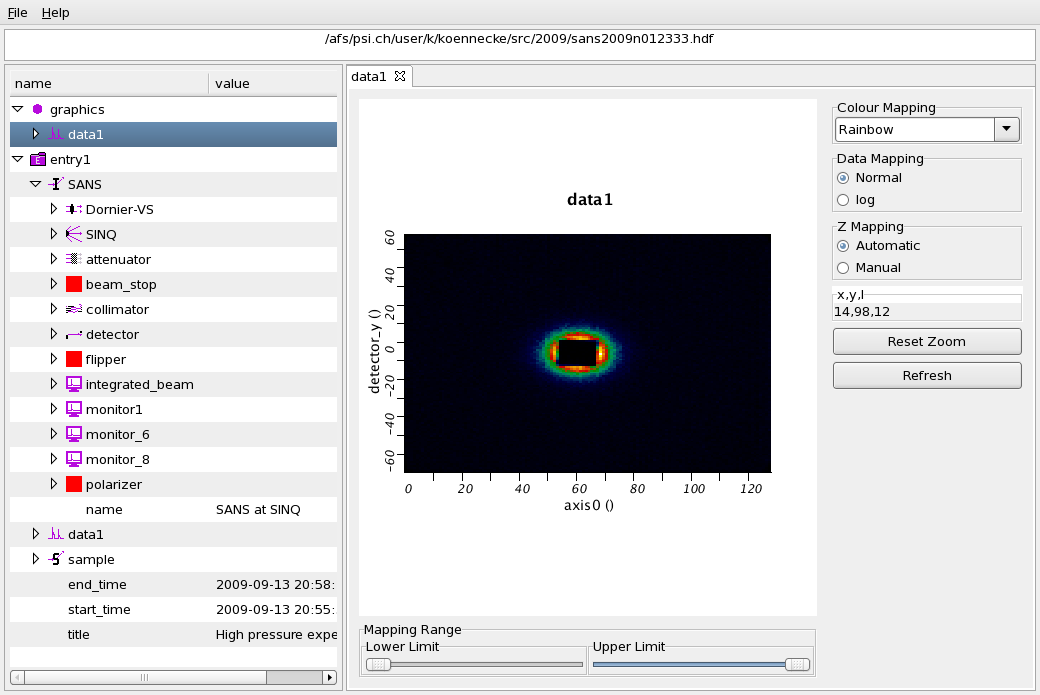
\includegraphics[width=0.75\textwidth]{NXplot.png}}\end{figure}
\end{frame}


\begin{frame} \frametitle{NeXus Conversions}
\begin{figure}[!ht]
\resizebox{7cm}{5cm}{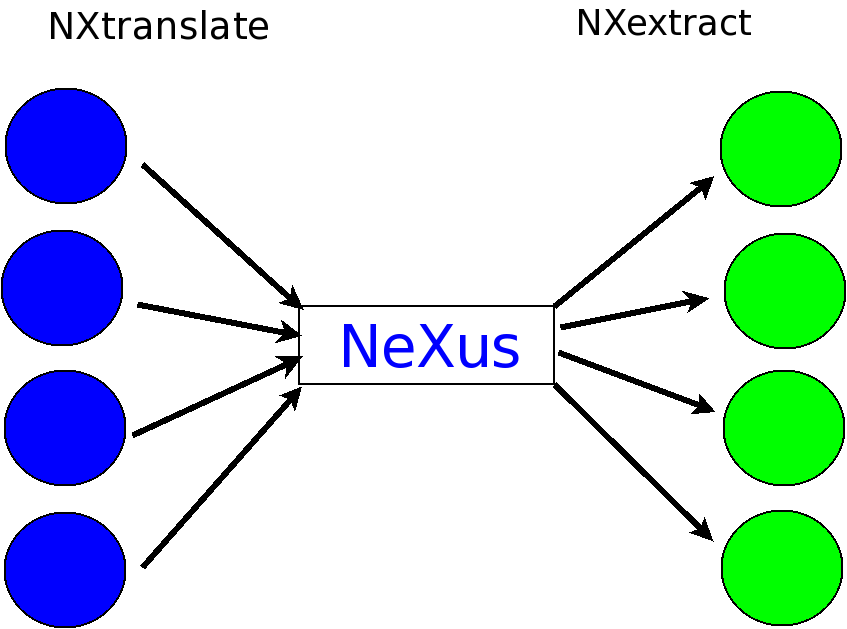
\includegraphics[width=0.75\textwidth]{nxswarch.png}}
\end{figure}
\end{frame}


\begin{frame} \frametitle{Other Systems Using NeXus}
\begin{itemize}
\item DANSE
\item DAVE
\item FABLE (ESRF)
\item ISAW
\item LAMP
\item openGenie
\item ICAT
\item Mantid
\item openGDA
\item All HDF tools
\end{itemize}
\end{frame}

\begin{frame} \frametitle{Who commits to NeXus? }
\begin{figure}[!ht]
\resizebox{7cm}{5cm}{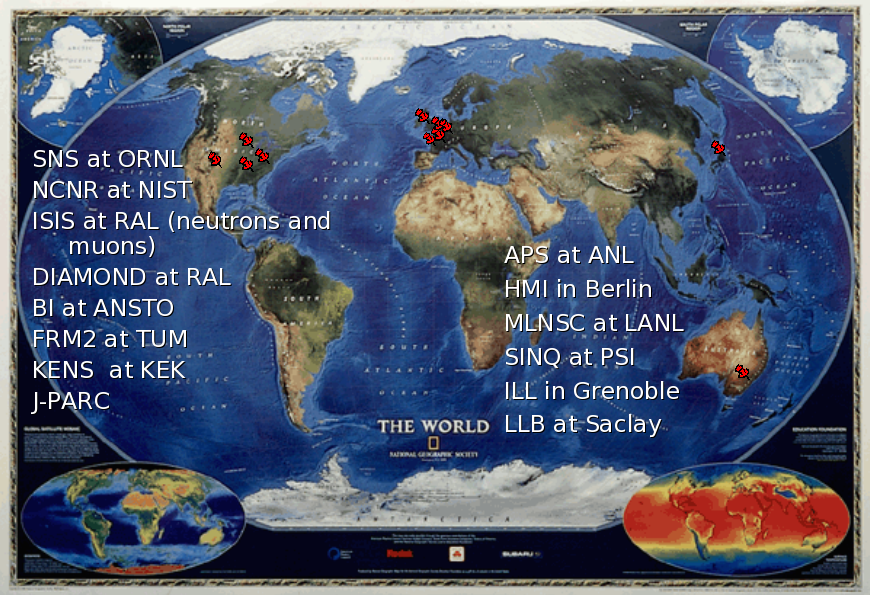
\includegraphics[width=0.75\textwidth]{nxworld.png}}\end{figure}
\end{frame}

\begin{frame} \frametitle{Data Format Challenges}
\begin{description}
\item<1->[Challenge 1] in science you are supposed to do new, non standard, things.  
 These of course cannot be easily cast into a standard.
\item<2->[Challenge 2] in order to establish a standard a lot of people need to agree
\item<3->[Challenge 3] a standard requires scarce scientific  programming resources for adoption 
\end{description}
\end{frame}

\begin{frame} \frametitle{Data Format Chances}
\begin{description}
\item<1->[Chance 1] By using a discoverable data format like NeXus, XML, HDF-5, people can at 
 least figure out  what is in the data file. 
\item<2->[Chance 2] Using predefined names from a dictionary gives meaning to the data in a file.
\item<3->[Chance 3] Using a shared API reduces learning costs and increases application stability.
\item<4->[Chance 4] With NeXus, HDF-5 plus professional programming techniques a DA application can 
 read any file which contains the required data.
\item<5->[Chance 5] Storing as much data as possible increases the likelihood that the needed 
 data is actually on file, even for unforeseen uses. 
\item<6->[Chance 6] Application Definitions
\end{description}
\end{frame}


\begin{frame} \frametitle{NeXus Interactions}
\begin{itemize}
\item PanData
\item Workshop: HDF5 as hyperspectral data format, January, ESRF
\item NeXus workshop at PSI, May
\item Upcoming: Data formats for HDR, DESY, end of october
\end{itemize}
\end{frame}

\begin{frame} \frametitle{PanData}
\begin{itemize}
\item European initiative for SSO, a shared data file catalog, DA etc
\item PanData needs a shared data format in order to make the catalog fly 
\item Works with NeXus 
\item Prompted us to have a project plan which we actually executed by now!
\item 5.5MM money
\end{itemize}
\end{frame}

\begin{frame} \frametitle{HDF5 as hyperspectral data format}
\begin{itemize}
\item End of January at ESRF, ca 30 participants
\item NeXus well received
\item Some confusion over a HDF-5 bug in 1.8
\item Demand to map imageCIF fully to NeXus in order to benefit from imageCIF ideas
\item Missing in NeXus to do full CIF mapping:
\begin{itemize}
\item Scaled data
\item CIF axis specification more accurate
\item Mapping to database concepts
\end{itemize}
\end{itemize}
\end{frame}


\begin{frame} \frametitle{NeXus for Synchrotrons}
\begin{itemize}
\item Workshop at PSI, 10-12 May
\item NeXus seen as HDF-5 with NeXus structures, no interest in API
\item Requests:
\begin{itemize}
\item NXsubentry
\item Scaled data
\item Simplified hierarchy for experts
\item Indicate image dimensions
\item Tree based higher level API
\end{itemize}
\end{itemize}
\end{frame}

\begin{frame} \frametitle{Threads Versus NeXus}
\begin{itemize}
\item Planned: NeXus is threadsafe when each thread has its own NXhandle
\item A little work needs to be done to arrive there
\item {\color{red}BUT:} HDF-5 serialises access, no performance gain!
\item Parallel HDF5, PHDF, with a different API
\item PHDF requires: MPI, MPI-IO, parallel file system
\item A new NeXus file driver for PHDF would be required
\item Will only be implemented when the community really wants it
\end{itemize}
\end{frame}

%% This meeting section


\begin{frame} \frametitle{Topics for this NIAC Meeting}
\begin{enumerate}
\item Constitution change: NIAC -- Tech, Chairman
\item Choose new  officers
\item NXsubentry
\item Scaled data
\item Coordinate systems
\item Next project plan
\item Simplified hierarchy, NXmeasurement
\item Event data
\item muSR NeXus
\end{enumerate}
\end{frame}


\begin{frame} \frametitle{Constitution Change}
\begin{itemize}
\item Observation: we make better progress when working in a smaller group of 
 experts
 \item Suggestion: Divide NIAC into two entities: 
\begin{itemize}
\item Full NIAC: votes officers, ratifies project plans, decides general directions  
\item Technical subcommittee: decides technical and implementation details, to be 
reviewed by full NIAC. Members are selected 
 on merit (contributed work) and approved by full NIAC
\end{itemize}
\item Full NIAC meets only any 2 years: requires extending the terms of officers
\end{itemize}
\end{frame}


\begin{frame} \frametitle{NXsubentry Rationale}
\begin{itemize}
\item Suggestion: add NXsubentry group below NXentry with the same structure as NXentry
\item Multi-method instrument
\begin{itemize}
\item Especially synchrotrons have instruments which combine multiple techniques in one experiment
\item Current NeXus would require separate NXentries for each technique
\item This becomes unnatural with the additional requirement to store multiple experiments in the same 
 file
\item Combining multiple application definitions in one NXentry would cause name collisions
\item The synchrotron people are willing to do the many links NXsubentry requires 
\end{itemize}
\item Add application definition compliant NXsubentries to existing files
\end{itemize}
\end{frame}


\begin{frame} \frametitle{NXsubentry}
\begin{tabbing}
\hspace*{1cm} \= \hspace*{1cm} \= \hspace*{1cm} \= \hspace*{1cm} \= \hspace*{1cm} \= \hspace*{1cm}\= \kill
entry:NXentry \\
 \>{\color{red} sas,NXsubentry}\\
 \>  \>sample:NXsample \\
\\
\> \>instrument:NXinstrument\\
\> \> \> source:NXsource\\
\> \> \> velocity\_selector:NXvelocity\_selector\\
\> \> \> detector:NXdetector \\
\> \> \> \>data[xsize,ysize], signal=1 (1)\\
\> \>control:NXmonitor\\
\> \> \>data\\
\> \>data:NXdata\\
\> \> \> link to (1)\\
\end{tabbing}
\end{frame}


\begin{frame} \frametitle{Scaled Data}
\begin{itemize}
\item NeXus stronly suggests storing physical values
\item Suggestion: allow scaled data for performance or other reasons
\item Implement through additional data attributes
\item NeXus stores arrays in C storage order
\item Suggestion: allow other orders
\item Implement through additional data attributes
\item NAPI will not implement the transforms
\end{itemize}
\end{frame}

\begin{frame} \frametitle{Scaled Data Attributes}
\begin{itemize}
\item scaling\_method: This is the indicator that a transformation of the Vraw data is 
   necessary. Scaling\_method can have one the following values:
\begin{itemize}
\item power: Vtrue = p0 + (Vraw/p1)**p2
\item logarithmic: Vtrue = p0 +p1*log(Vraw*p2)   
\item  polynomial: Vtrue = p0 + p1*Vraw + p2*Vraw*Vraw + p3*Vraw*Vraw*Vraw ....
\item To be expanded?
\item Or give the formula?
\end{itemize}
\item 0, p1, p2, ... Float attributes as parameters
\item scaled\_units: units after scaling
\item Offset, stride
\end{itemize}
\end{frame}


\begin{frame} \frametitle{Coordinate Systems}
\begin{itemize}
\item Another look on coordinate systems
\item NeXus:
\begin{itemize}
\item Simple, polar coordinates using angles and distances
\item Absolute McStas coordinates using NXgeometry
\end{itemize}
\item imageCIF
\begin{itemize}
\item Arbitrary axis allowed
\item Contains information to build transformation matrices
\end{itemize}
\end{itemize}
\end{frame}

\begin{frame} \frametitle{Transformation Matrices}
\begin{math}
T = \left( \begin{array}{cccc}
1 & 0 & 0 & x\\
0 & 1 & 0 & y\\
0 & 0 & 1 & z\\
0 & 0 & 0 & 1\\
\end{array} \right)
\end{math}

\begin{math}
\onslide+<2-> 
R = \left( \begin{array}{cccc}
r11 & r12 & r13 & 0\\
r21 & r22 & r23 & 0\\
r31 & r32 & r33 & 0\\
0 & 0 & 0 & 1\\
\end{array} \right)
\end{math}

\end{frame}

\begin{frame} \frametitle{Combining Transformations}
\begin{figure}[!ht]
\resizebox{7cm}{5cm}{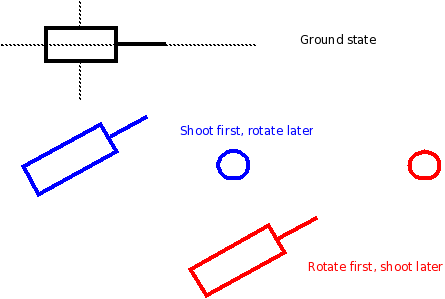
\includegraphics[width=0.75\textwidth]{rotcombi.png}}\end{figure}
\end{frame}

\begin{frame} \frametitle{Some Properties}
\begin{itemize}
\item Transformations can be combined by matrix multiplications
\item Individual matrices can be derived by looking at the situation when everything else is 0
\item Absolute positions can be obtained by multiplying the resulting matrix with its transpose
\item Defines new coordinate systems at components
\item CIF contains a duplication: vector, offset scheme 
\end{itemize}
\end{frame}

\begin{frame} \frametitle{What Use Is This?}
\begin{itemize}
\item Allows to calculate absolute positions of components in the laboratory coordinate systems
\item Can directly convert from a detector coordinate system to  
 vectors in Lab coordinate system
\item Calculate things like impact of primary beam on detector, SAS
\item Allows arbitray axis to be expressed
\item Intuitively describe an instrument with angles and translations and still be able
 to recover absolute coordinates
\end{itemize}
\end{frame}


\begin{frame} \frametitle{Information Required}
\begin{description}
\item[type] rotation or translation
\item[direction] vector around which rotated or translated
\item[value] The angle of rotation or the length of translation
\item[dependency] The order of operations to place a component
\end{description}
\end{frame}


\begin{frame} \frametitle{Use For NeXus}
\begin{itemize}
\item Use to document existing axis and polar coordinate system better
\item Permits arbitrary axis to be defined
\item Allows construction of transformation matrices and gain the advantages of using them
\item Allows to express an instrument intuitively as a sequence of translations and 
 rotations AND be able to reconstruct absolute positions
\item The objective is to allow a full mapping from imageCIF to NeXus and back
\end{itemize}
\end{frame}

\begin{frame} \frametitle{NeXus Axis Mapped}
\begin{itemize}
\item rotation\_angle, polar\_angle, rotate 0 1 0
\item azimuthal\_angle, rotate 0 0 1
\item distance, translate 0 0  1
\item chi, rotate 0 0 1
\item phi rotate, 0 1 0
\item NeXus polar coordinate system: rotate azimuthal\_angle, rotate polar\_angle, 
 translate by distance
\end{itemize}
\end{frame}

\begin{frame} \frametitle{Axis Suggestions for NeXus}
\begin{itemize}
\item NeXus stays with the McStas Laboratory coordinate system 
\item NeXus strongly encourages to use the named and documented NeXus 
  axis
\item Allow attributes type, direction in order to support arbitrary axis 
\item Add aequatorial\_angle as a name to appear in base classes for 
 rotation 1 0 0. 
\item Add y\_translation (translate 0 1 0) 
 and x\_translation (translate 1 0 0) to base classes.   
\end{itemize}
\end{frame}

\begin{frame} \frametitle{Expressing Axis Dependency in NeXus}
\begin{itemize}
\item Implied: use existing NeXus coordinate system
\item dependson attribute pointing to depending axis
\item transform field in base classes which becomes a comma separated list of 
 the path to the transformations required to position this component
\item Create a special container to hold axis dependencies, NXdependency, to 
 collect the dependencies in one place for easy access. This is what CIF does
\end{itemize}
\end{frame}

\begin{frame} \frametitle{Dependons Option}
\begin{tabbing}
\hspace*{1cm} \= \hspace*{1cm} \= \hspace*{1cm} \= \hspace*{1cm} \= \hspace*{1cm} \= \hspace*{1cm}\= \kill
\>sample,NXsample\\
\> \>rotation\_angle\\
\> \>chi (dependson rotation\_angle)\\
\> \>phi (dependson phi)\\
\end{tabbing}
\end{frame}

\begin{frame} \frametitle{Transform Option}
\begin{tabbing}
\hspace*{1cm} \= \hspace*{1cm} \= \hspace*{1cm} \= \hspace*{1cm} \= \hspace*{1cm} \= \hspace*{1cm}\= \kill
\>sample,NXsample\\
\> \>rotation\_angle\\
\> \>chi \\
\> \>phi \\
\> \>transform = rotation\_angle,chi,phi \\
\end{tabbing}
\end{frame}


\begin{frame} \frametitle{Separate Group Option}
\begin{tabbing}
\hspace*{1cm} \= \hspace*{1cm} \= \hspace*{1cm} \= \hspace*{1cm} \= \hspace*{1cm} \= \hspace*{1cm}\= \kill
\>sample,NXsample\\
\> \>rotation\_angle\\
\> \>chi \\
\> \>phi \\
\>dependency,NXdependency\\
\> \>sample/chi = \\
\> \> \>sample/rotation\_angle\\
\> \>sample/phi =\\
\> \> \> sample/chi\\
\> \>instrument/detector/x\_translation = \\
\> \> \>instrument/detector/distance\\
\> \>instrument/detector/distance = \\
\> \> \>instrument/detector/polar\_angle\\
\end{tabbing}
\end{frame}




\begin{frame} \frametitle{NXmeasurement}
\begin{tabbing}
\hspace*{1cm} \= \hspace*{1cm} \= \hspace*{1cm} \= \hspace*{1cm} \= \hspace*{1cm} \= \hspace*{1cm}\= \kill
\>entry,NXentry\\
\> \>measurement,NXmeasurement\\
\> \> \>positions:NXpositioner\\
\> \> \> \>om \\
\> \> \> \>two\_theta\\
\> \> \>scalars:NXscalar\\
\> \> \> \>title\\
\> \> \> \>wavelength\\
\> \> \>data:NXdata\\
\> \> \> \>detector1\\
\> \> \> \>mca5\\
\end{tabbing}
\end{frame}


\begin{frame} \frametitle{Ideas for Project Plan 2012}
\begin{itemize}
\item Refinement of application definitions with communities
\begin{itemize}
\item Collect community feedback
\item Release of NXDL, base classes and application definitions 1.0 
\end{itemize}
\item nxvalidate 1.0
\item Overhaul of documentation: Manual, NAPI, WWW-site
\item OO base classes?
\item Higher level NeXus-APIs?
\end{itemize}
\end{frame}


\end{document}


\begin{frame}
\frametitle{The Predicament of the Traveling Scientist}
\begin{itemize}
\item<1->A different data format wherever she goes
\item<2->Spends lots of time converting formats or writing readers
\item<3->Waits even longer to load data from inefficient data formats
\item<4->DA requires N files in different  formats, notes, local knowledge 
\item<5->Cannot read her collaborators data
\item<6->Has to keep extra information in yet another form
\end{itemize}
\end{frame}


\begin{frame} \frametitle{Conclusion }
\begin{itemize}
\item NeXus is a mature and capable data format
\item There is no other standard then NeXus on the horizon
\item New things are developed with NeXus everywhere, uptake at established sites is slow
\item You are invited to join the NIAC and contribute to NeXus 
\item More information: http://www.nexusformat.org (outdated, but working on it)
\end{itemize}
\end{frame}


\begin{frame} \frametitle{Example Files}
\end{frame}

\begin{frame} \frametitle{Storing Single Data Items }
\begin{itemize}\item Units have to specified
\item Locating axis, by example:
\begin{itemize}\item counts(two\_theta, time\_of\_flight), attributes: signal=1
\item two\_theta, attributes: axis=1, axis=primary 
\item time\_of\_fligth, attributes: axis=2, axis=primary
\end{itemize}\end{itemize}
\end{frame}

\begin{frame} \frametitle{NXtranslate }
\begin{itemize}\item Anything to NeXus converter:
\begin{itemize}\item Binary dump
\item FRM2
\item IPNS run
\item NeXus
\item Spec
\item XML
\end{itemize}\item Uses XML based translation file to control translation
\item Extendable via plugins
\end{itemize}
\end{frame}

\begin{frame} \frametitle{NXextract}
\begin{itemize}
\item Extracts NeXus files to binary or ASCII
\item Uses XML template file to control conversion
\item Contributed by Stephane Poirier, SOLEIL 
\end{itemize}
\end{frame}

\begin{frame} \frametitle{Another Way to use NeXus/HDF-5}
\begin{enumerate}
\item Use NXopenpath(hfil,path) to access the data in file, use introspection to 
 find out about dimensions
\item Have a dictionary mapping what you need for DA to paths
\item Keep the dictionary in a separate file
\item When you encounter a different file, just edit the dictionary file 
\end{enumerate}
\end{frame}

\begin{frame} \frametitle{McStas Coordinate System }
\begin{figure}[!ht]
\resizebox{7cm}{5cm}{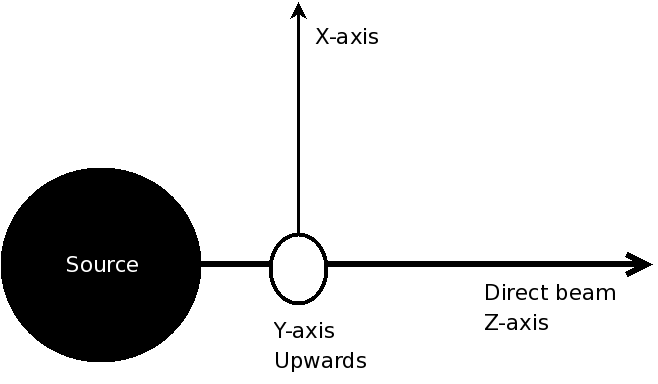
\includegraphics[width=0.75\textwidth]{mcstas.png}}\end{figure}
\end{frame}

\begin{frame} \frametitle{NeXus Simple Coordinate System }
\begin{figure}[!ht]
\resizebox{7cm}{5cm}{\includegraphics[width=0.75\textwidth]{polplane.png}}\end{figure}
\end{frame}




\begin{frame} 
\frametitle{NeXus Endorsement }
\begin{table}[!ht]
\begin{tabular}{|c|c|c|}
\hline
SNS at ORNL & SINQ at PSI\\ \hline
 NCNR at NIST & ISIS at RAL\\ \hline
 Diamond at RAL&Opal at ANSTO\\ \hline
FRM2 at TUM&KENS at KEK\\ \hline
J-Parc & IPNS at ANL\\ \hline
APS at ANL& HMI in Berlin\\ \hline
MLNSC at LANL& LLB in Saclay\\ \hline
\end{tabular}\end{table}
\end{frame}




\begin{frame} \frametitle{NeXus Levels }
\begin{enumerate}\item Physical file format
\item API for accessing files
\item Structure for organizing data in files
\item Rules for storing individual data items
\item Component and application definitions
\end{enumerate}
\end{frame}

\begin{frame} \frametitle{NXtranslate }
\begin{itemize}\item Anything to NeXus converter:
\begin{itemize}\item Binary dump
\item FRM2
\item IPNS run
\item NeXus
\item Spec
\item XML
\end{itemize}\item Uses XML based translation file to control translation
\item Extendable via plugins
\end{itemize}
\end{frame}

\begin{frame} \frametitle{NXextract}
\begin{itemize}
\item Extracts NeXus files to binary or ASCII
\item Uses XML template file to control conversion
\item Contributed by Stephane Poirier, SOLEIL 
\end{itemize}
\end{frame}


\begin{frame}[fragile] 
\frametitle{Aside: CIF Hierarchies}
CIF uses Hierarchies too, but hides them:
\uncover<1->{
\begin{semiverbatim}
\_exptl\_crystal\_description        plate\newline
\_exptl\_crystal\_colour             colourless\newline
\_exptl\_crystal\_size\_max           0.30
\end{semiverbatim}
}
\uncover<2>{
\begin{semiverbatim}
/exptl/crystal/description        plate\newline
/exptl/crystal/colour             colourless\newline
/exptl/crystal/size/max           0.30
\end{semiverbatim}
}

\end{frame}

\begin{frame}
\frametitle{Why a Common Dataformat? }

\begin{itemize}\item Today: 
\begin{itemize}\item Lots of different data formats
\item Time wasted converting data
\item Old formats no longer capable of delivering for new high throughput detectors
\item Difficult to add additional data
\item Often, for DA multiple different files needed
\item Badly documented formats
\end{itemize}\item Tomorrow, with NeXus:
\begin{itemize}
\item Single, efficient, platform independent data format
\item All information in one file
\item Self describing
\item Extendable
\end{itemize}
\end{itemize}
\end{frame}

\begin{frame} \frametitle{Using Tabbing for Hierarchy}
\begin{tabbing}
\hspace*{1cm} \= \hspace*{1cm} \= \hspace*{1cm} \= \hspace*{1cm} \= \kill
entry:NXentry \\
 \>sample:NXsample \\
 \> \> rotation\_angle[NP], axis=1 (1) \\
\\
 \>instrument:NXinstrument\\
 \> \> detector:NXdetector \\
 \> \> \>data[NP], signal=1 (2)\\
 \>data:NXdata\\
 \> \> link to (1)\\
 \> \> link to (2)\\
\end{tabbing}
\end{frame}
